\chapter{Construction of a Sound Robot}
\label{chap_design}

In the last chapter, I showed that a toy robot with a fictional back story could elicit empathy. Now, I will describe the design and construction of a zoomorphic social robot that has the ability to autonomously create its own life story. The robot can learn to mimic sounds it hears and improve its imitations with repetition. 



   \begin{figure}[thpb]
      \centering
      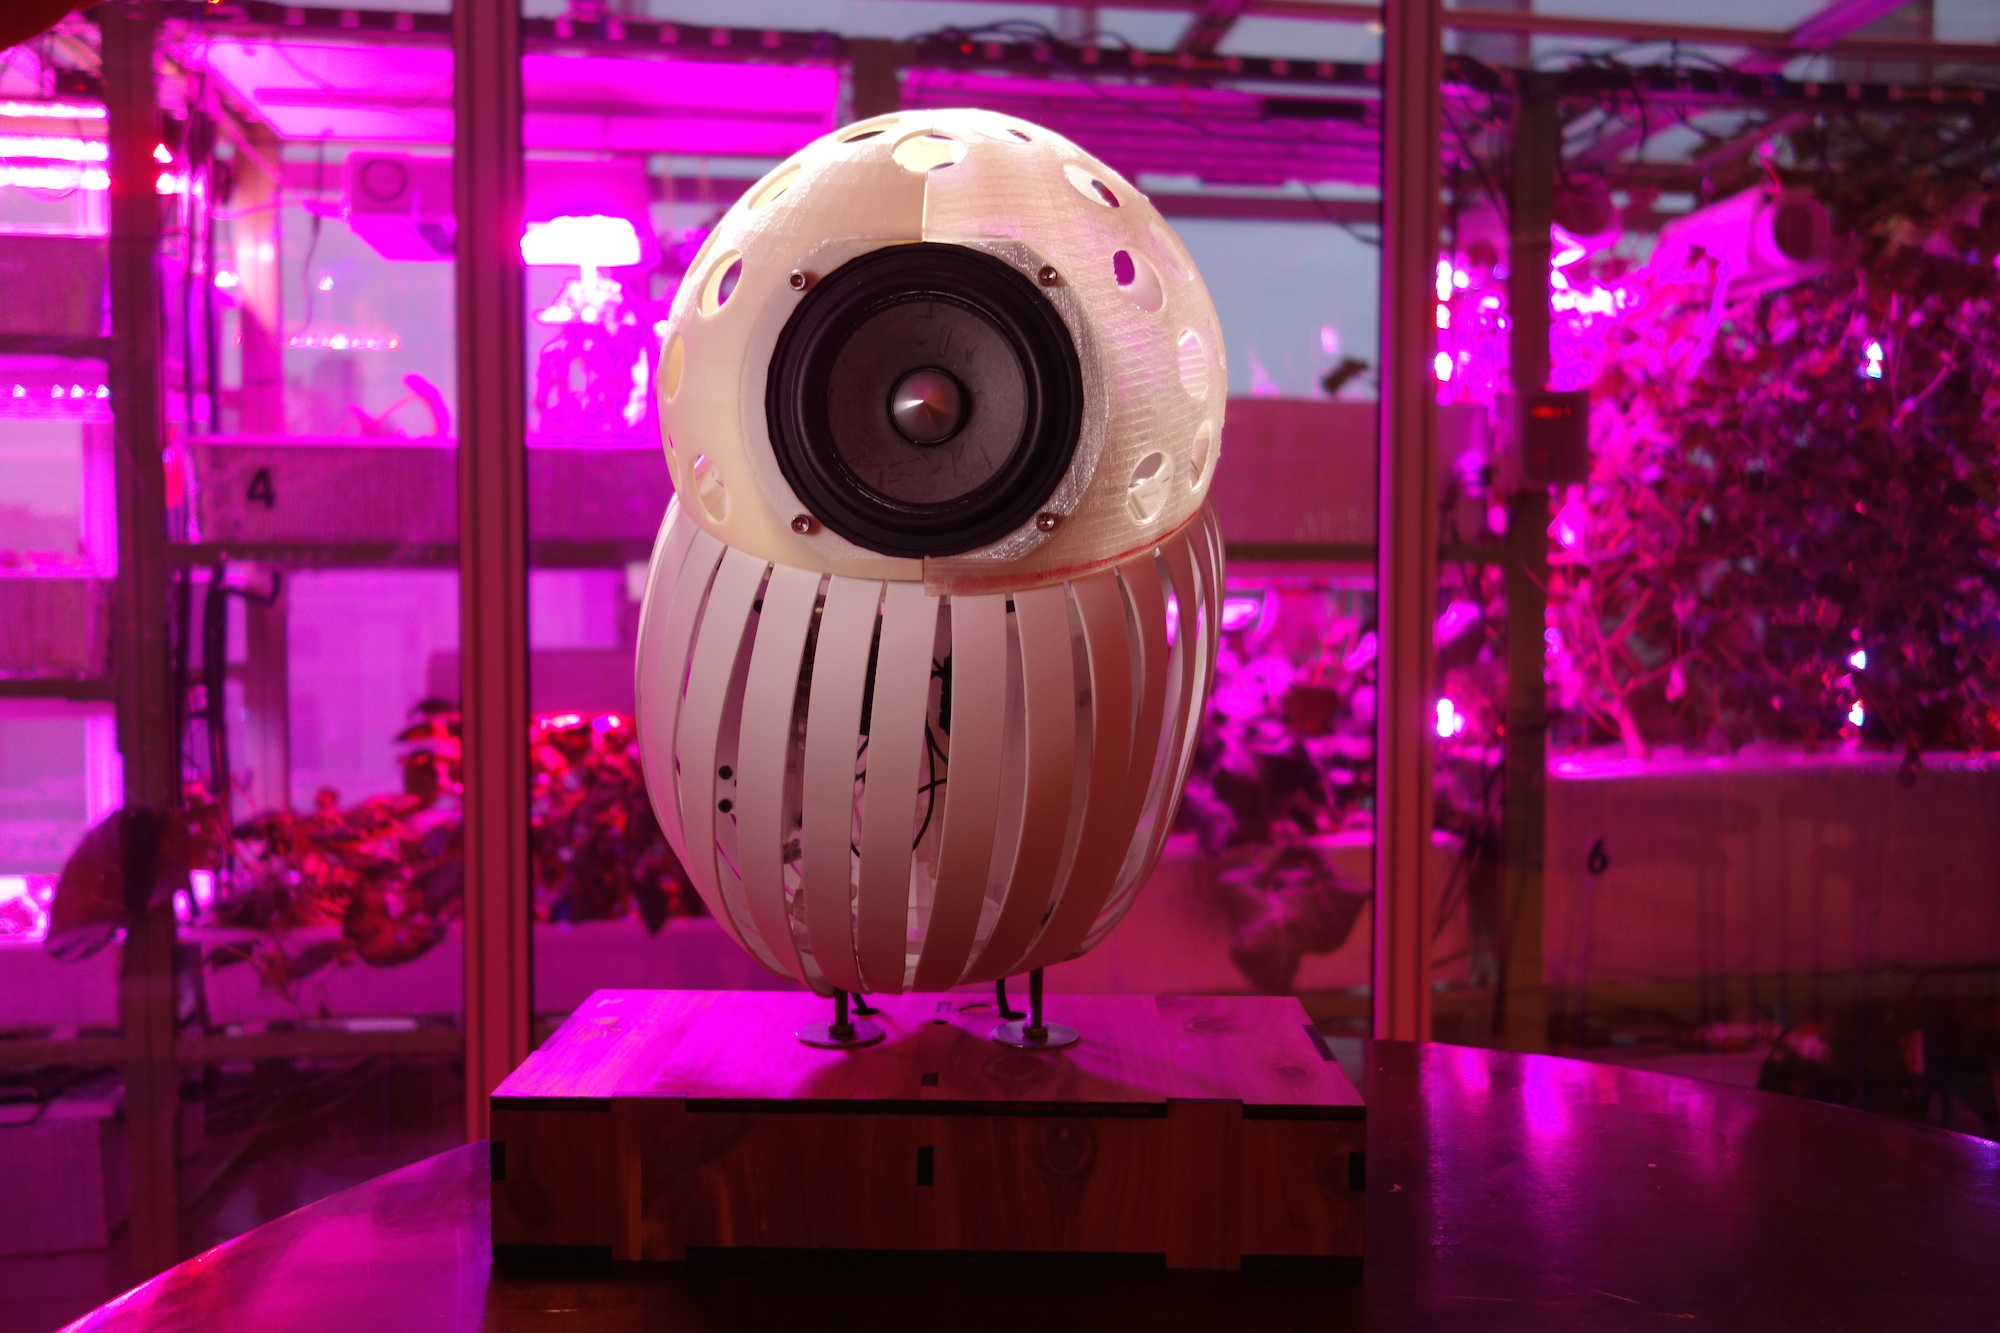
\includegraphics[width=4.6in]{figures/design/parrot_purple.JPG}
      \caption{Ewol the Electric Owl, the sound robot described in this chapter}
      \label{fig_parrot_purple}
   \end{figure}
   

\section{Why a Sound Robot?}

An important design goal for a life-story robot is that it should experience the world in ways we do and change perceptibly from that experience. A sound robot has certain properties that make it attractive for the purpose of this thesis.  Sound allows for human oriented perception that is rich in information ranging from environmental sounds, to thoughts as expressed as words, taking in along the way emotions and speech patterns unique to individuals. Recent advances in technologies such as sound localization, speaker identification, and particularly speech recognition, allow the construction of a robot that can obtain salient information from sound. 

A sound based robot can also be optionally ambient, that is to say, if needed it can experience the world by being merely present in an environment without requiring direct human intervention for the experiences. This allows the robot to have experiences autonomously over long time periods. 

A sound robot can make use of a familiar interaction model, namely how humans typically interact with avian pets such as parrots. People's expectations of intelligence and emotional expression are lower for birds compared to cats or dogs which makes design goals for a bird-like robot more modest. In addition to establishing low expectations for interaction, utilizing the avian companion model solves a thorny problem for robots: power distribution. A robot of the avian persuasion can be plausibly restricted to sitting on a perch which would allow for power and data connections. 


\section{Design Process}

   \begin{figure}[thpb]
      \centering
      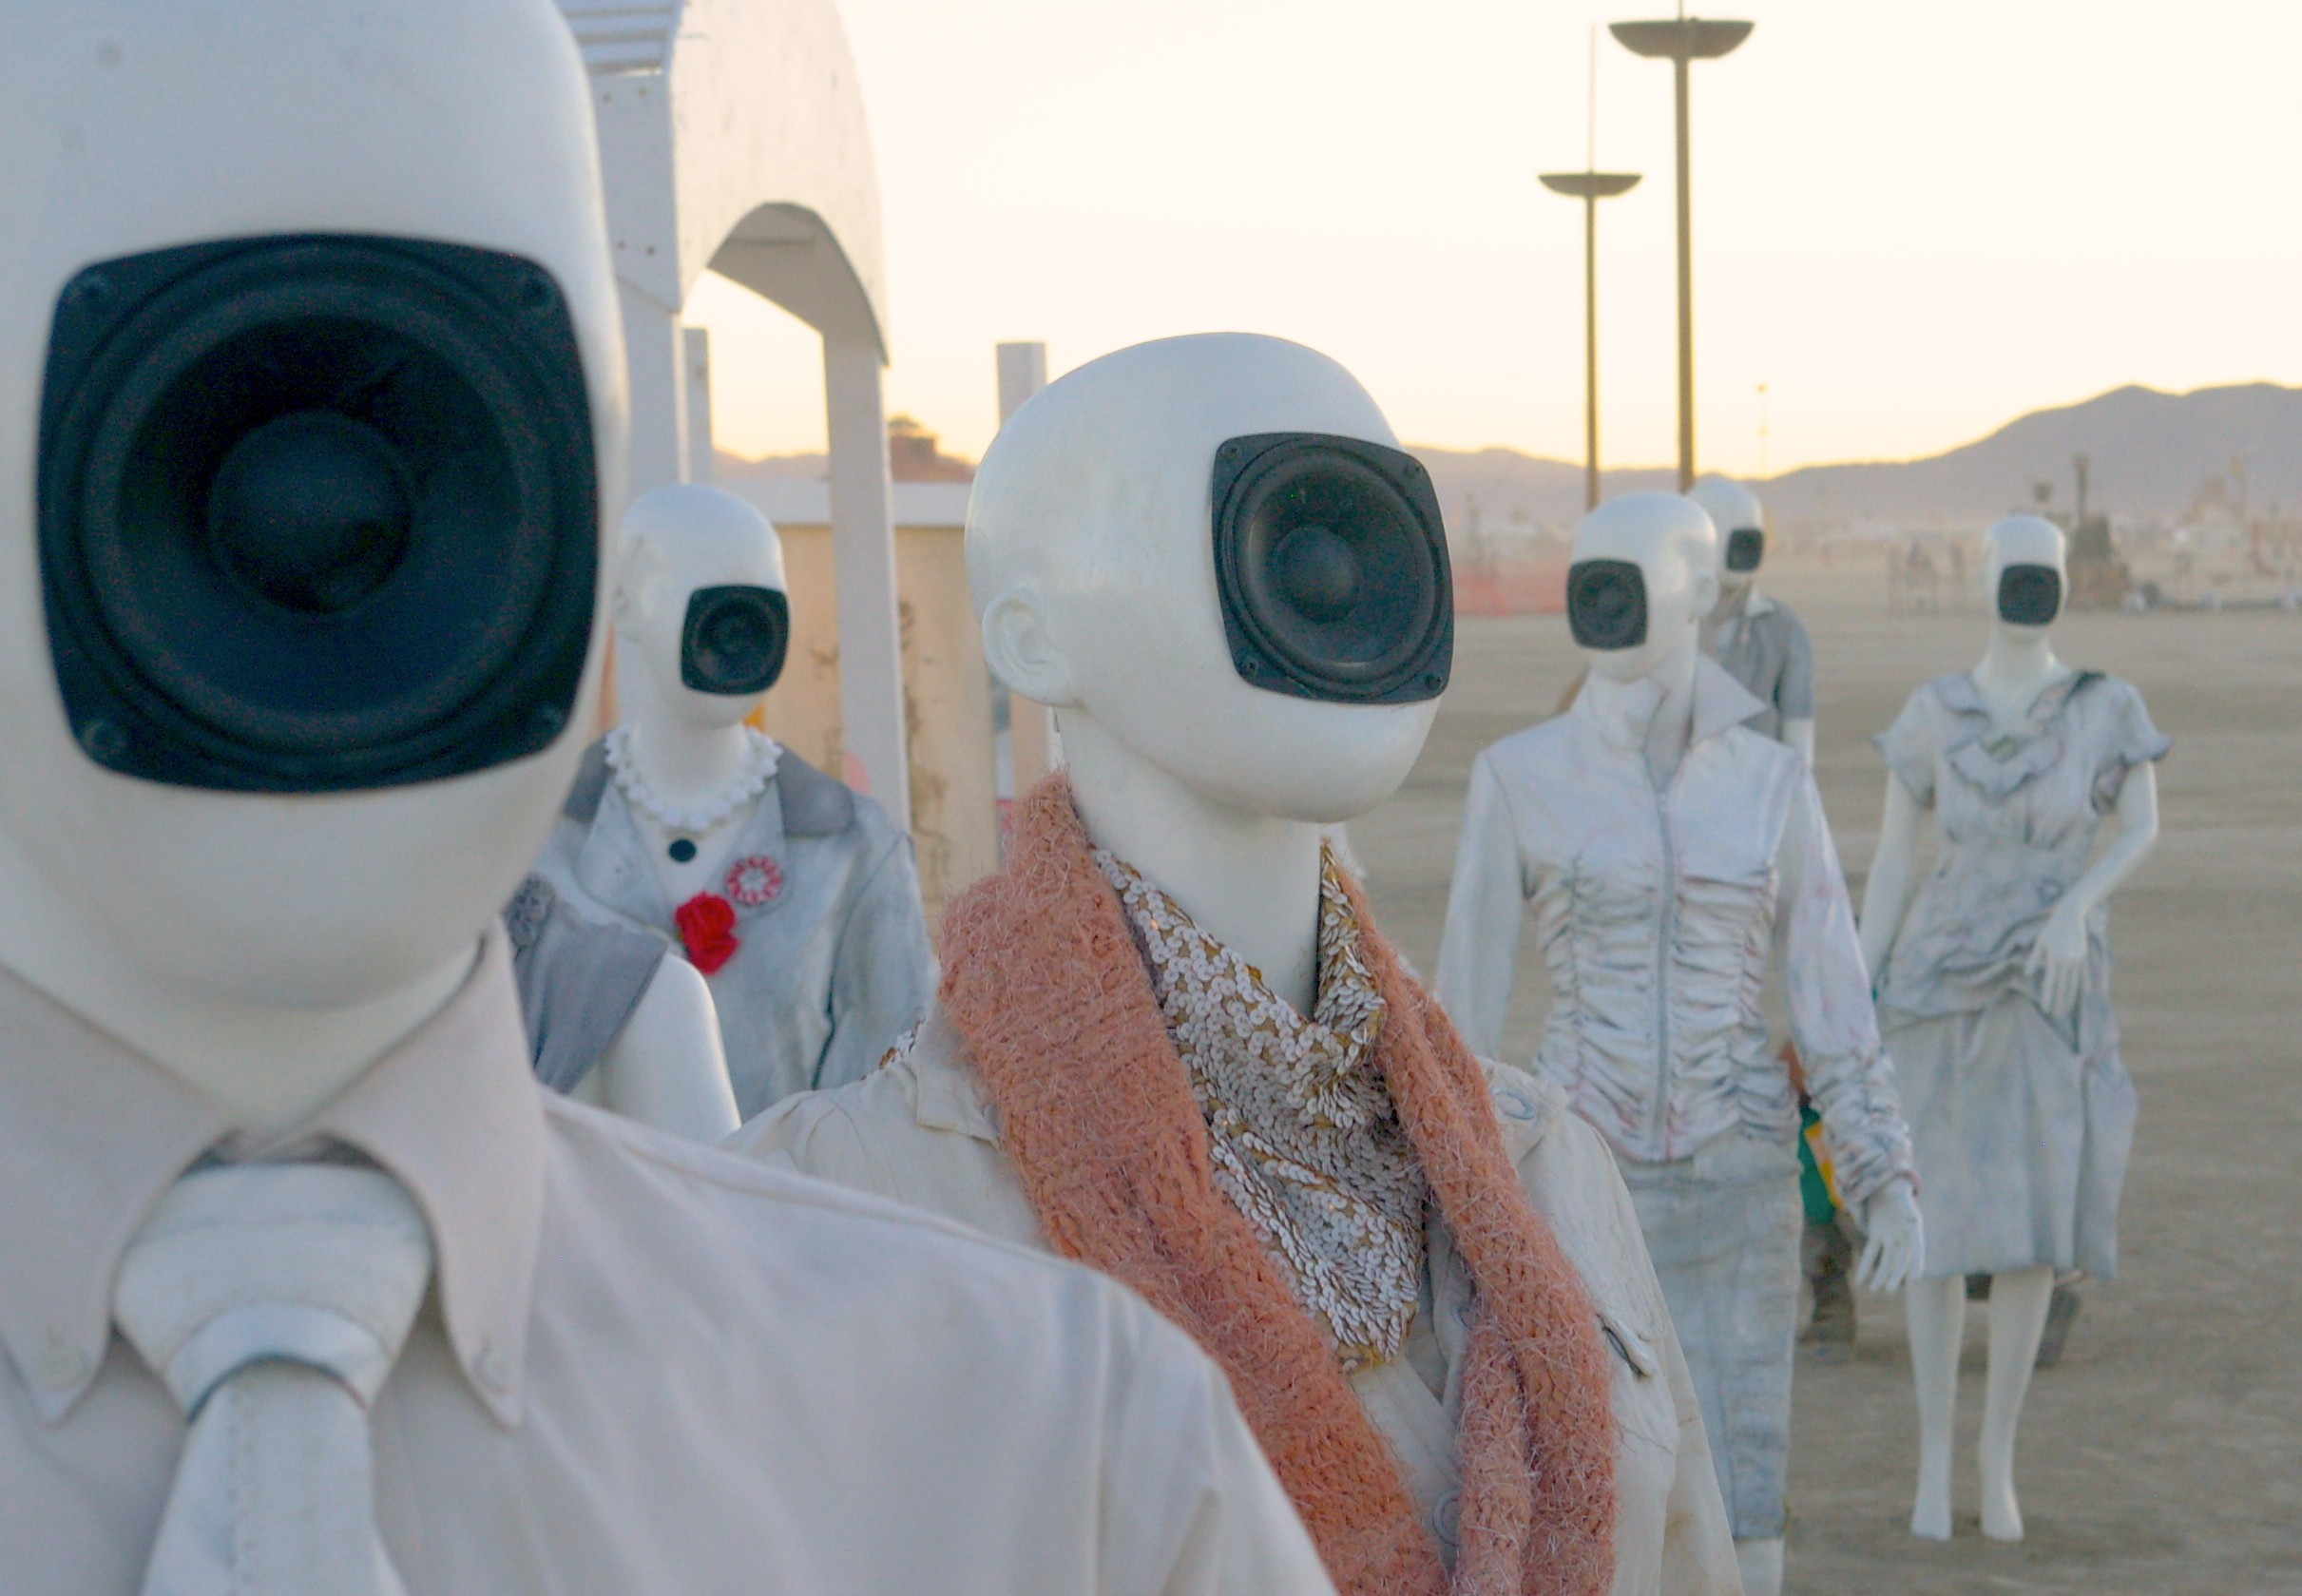
\includegraphics[width=4.6in]{figures/design/burning_man_speakers_sm.jpg}
      \caption{Mannequins with speakers by unknown artist at Burning Man 2010, the inspiration for the speaker-as-face design for my robot}
      \label{fig_burning_man_speakers_sm}
   \end{figure}
   



   \begin{figure}[thpb]
      \centering
      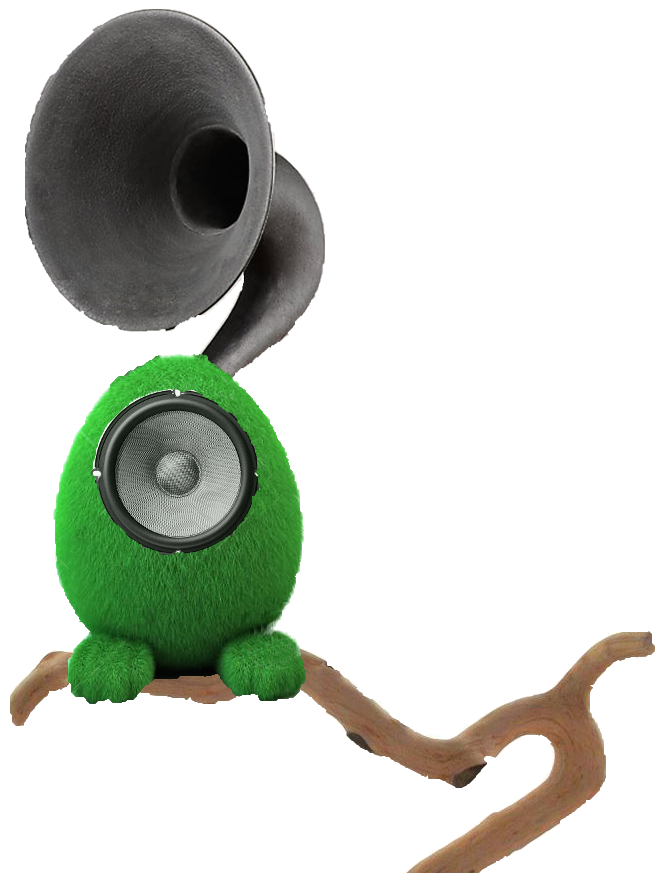
\includegraphics[width=3in]{figures/design/green_blob2.png}
      \caption{Early design for the robot with exaggerated sound features}
      \label{fig_green_blob2}
   \end{figure}


   \begin{figure}[thpb]
      \centering
      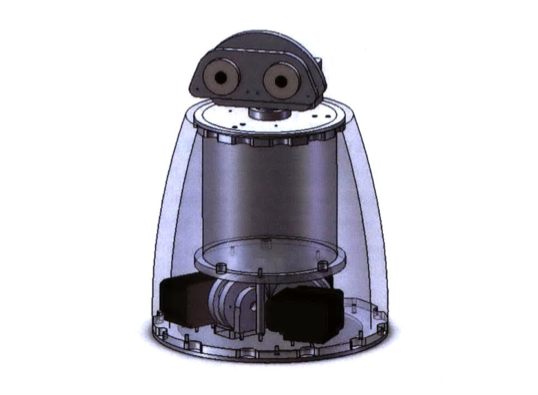
\includegraphics[width=4in]{figures/design/tofu_design.png}
      \caption{Ryan Wistort's Tofu showing squash stretch mechanism \cite{wistort_tofu_draw}. Three servos in the base of the robot pulled on cables that compressed a central column of bedding foam. Tofu's motion and mechanism inspired the design of my sound robot.}
      \label{fig_tofu_design}
   \end{figure}


  \begin{figure}[thpb]
      \centering
      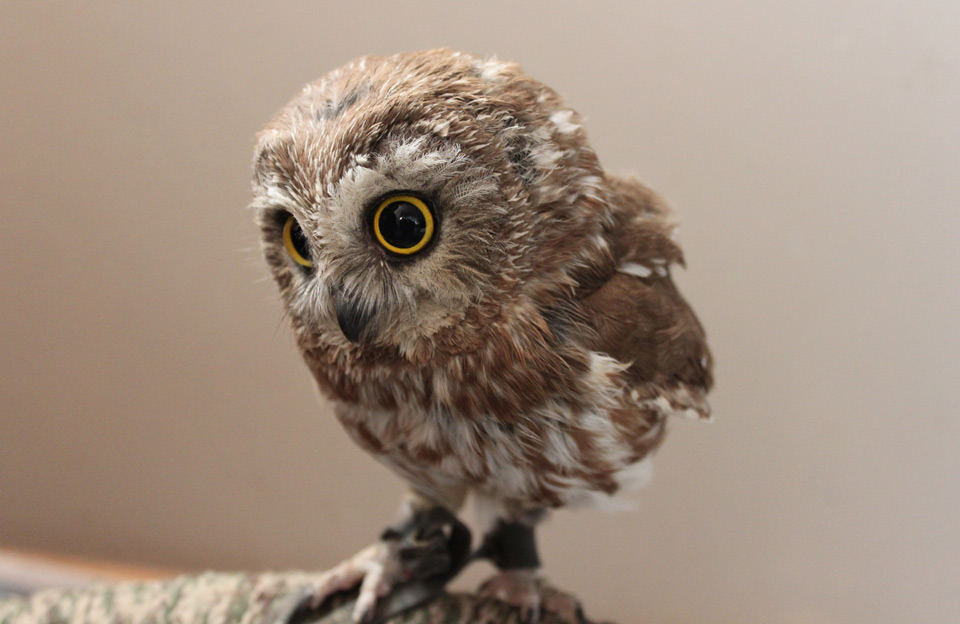
\includegraphics[width=4.6in]{figures/design/owl_inspiration.jpg}
      \caption{Juvenile owl used as an inspiration for the sound robot's form design.}
      \label{fig_owl_inspiration}
   \end{figure}

One of the primary physical design goals was to indicate through visual clues that the robot supported only sound based interaction. To that end, the robot should have exaggerated sound features and, rather unusually for social robots, no discernible eyes. Moreover, to suggest a parrot-like interaction, its form and movement should evoke those of a bird. 

Figure \ref{fig_green_blob2} shows my initial design for the sound robot. The body is based around a blob shape that can squash and stretch much like Wistort's Tofu robot (See Figure \ref{fig_tofu_design}) \cite{wistort_tofu_draw}. The green fur covering is evocative of a parrot. Inspired by a moving work of art which used speakers for faces of mannequins (Figure \ref{fig_burning_man_speakers_sm}), the main feature of the robot's face is a speaker. A large gramophone horn stands in for an over-sized ear trumpet. The overall hybrid mechanical organic form seemed suitable for a robot that is aspiring to be life-like. The whole robot is mounted on a branch which route power and data. 

Life-like motion, as discussed earlier, is a key contributor to robot's believability.\marginpar{

      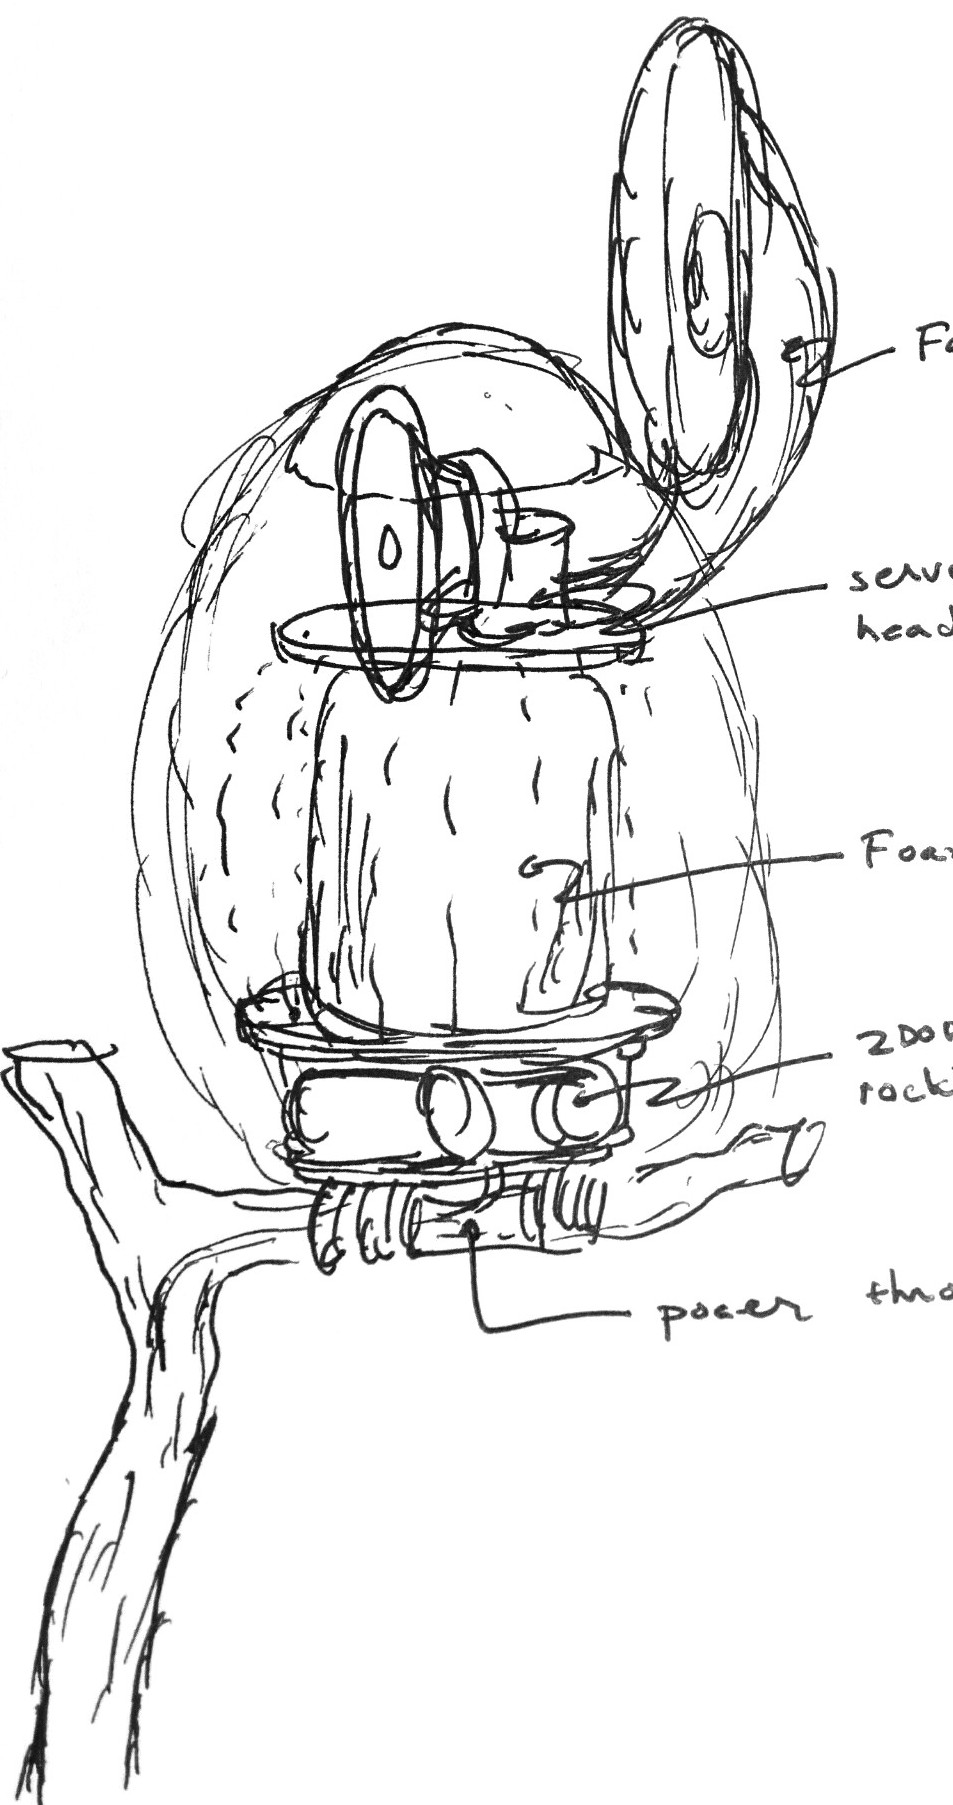
\includegraphics[width=\marginparwidth]{figures/design/hand_drawn_green_blob2.jpg}
      Sketch of potential mechanisms.
      %\caption{Juvenile owl used as an inspiration for the sound robot's form design.}
      \label{fig_design_hand_drawn}

   

} In this design, the robot would be able to do a breathing motion while idling, puff up when it is speaking, rock side to side to suggest excitement, lean forward to show interest, lean back to indicate fear, turn its head to look around, and cock its head to listen. Much like the use of ears in other social robots, the independent movement of the trumpet could be used for expressing affect. 

While revising this initial design, for aesthetic reasons, I changed the form to be closer to that of a juvenile owl (Figure \ref{fig_owl_inspiration}) than a parrot. The trumpet was sacrificed for simplicity of construction. In response to feedback from early testing, the robot got a foam skin that exposed the internal structure instead of fur, shifting the overall design to be more mechanical than organic. 


\section{Physical Construction}

The mechanism for the sound robot is fairly simple \footnote{I worked on the physical construction with Andres Salgado-Bierman, an undergraduate researcher. Andres was responsible for an early version of the linear actuator and the skin for the robot. I am indebted to Andres for his help, and also to Arthur Preton, Matt Carney, Young Dae and Harald Quintas-Baz for feedback on the mechanical design.}. The robot has four degrees of freedom, three of which are used for animating the body and one for turning the head. 

\subsection{Body}

The body of the robot consists of two parallel plates connected by three linear actuators. Extensions or contractions of the actuators can translate the plates up and down, or pitch forward and backward, or roll left and right. As the plates move relative to each other, they stretch or compress a foam skin changing the apparent shape and size of the body while keeping its volume constant. 

The bottom plate is mounted at an angle to the ground so that the axis of the body tilts forward at rest. Due to this forward tilt, an extension of the plates causes the robot to stretch forward towards the user, and a retraction to shrink away allowing it to express interest or fear. 






   \begin{figure}[thpb]
      \centering
      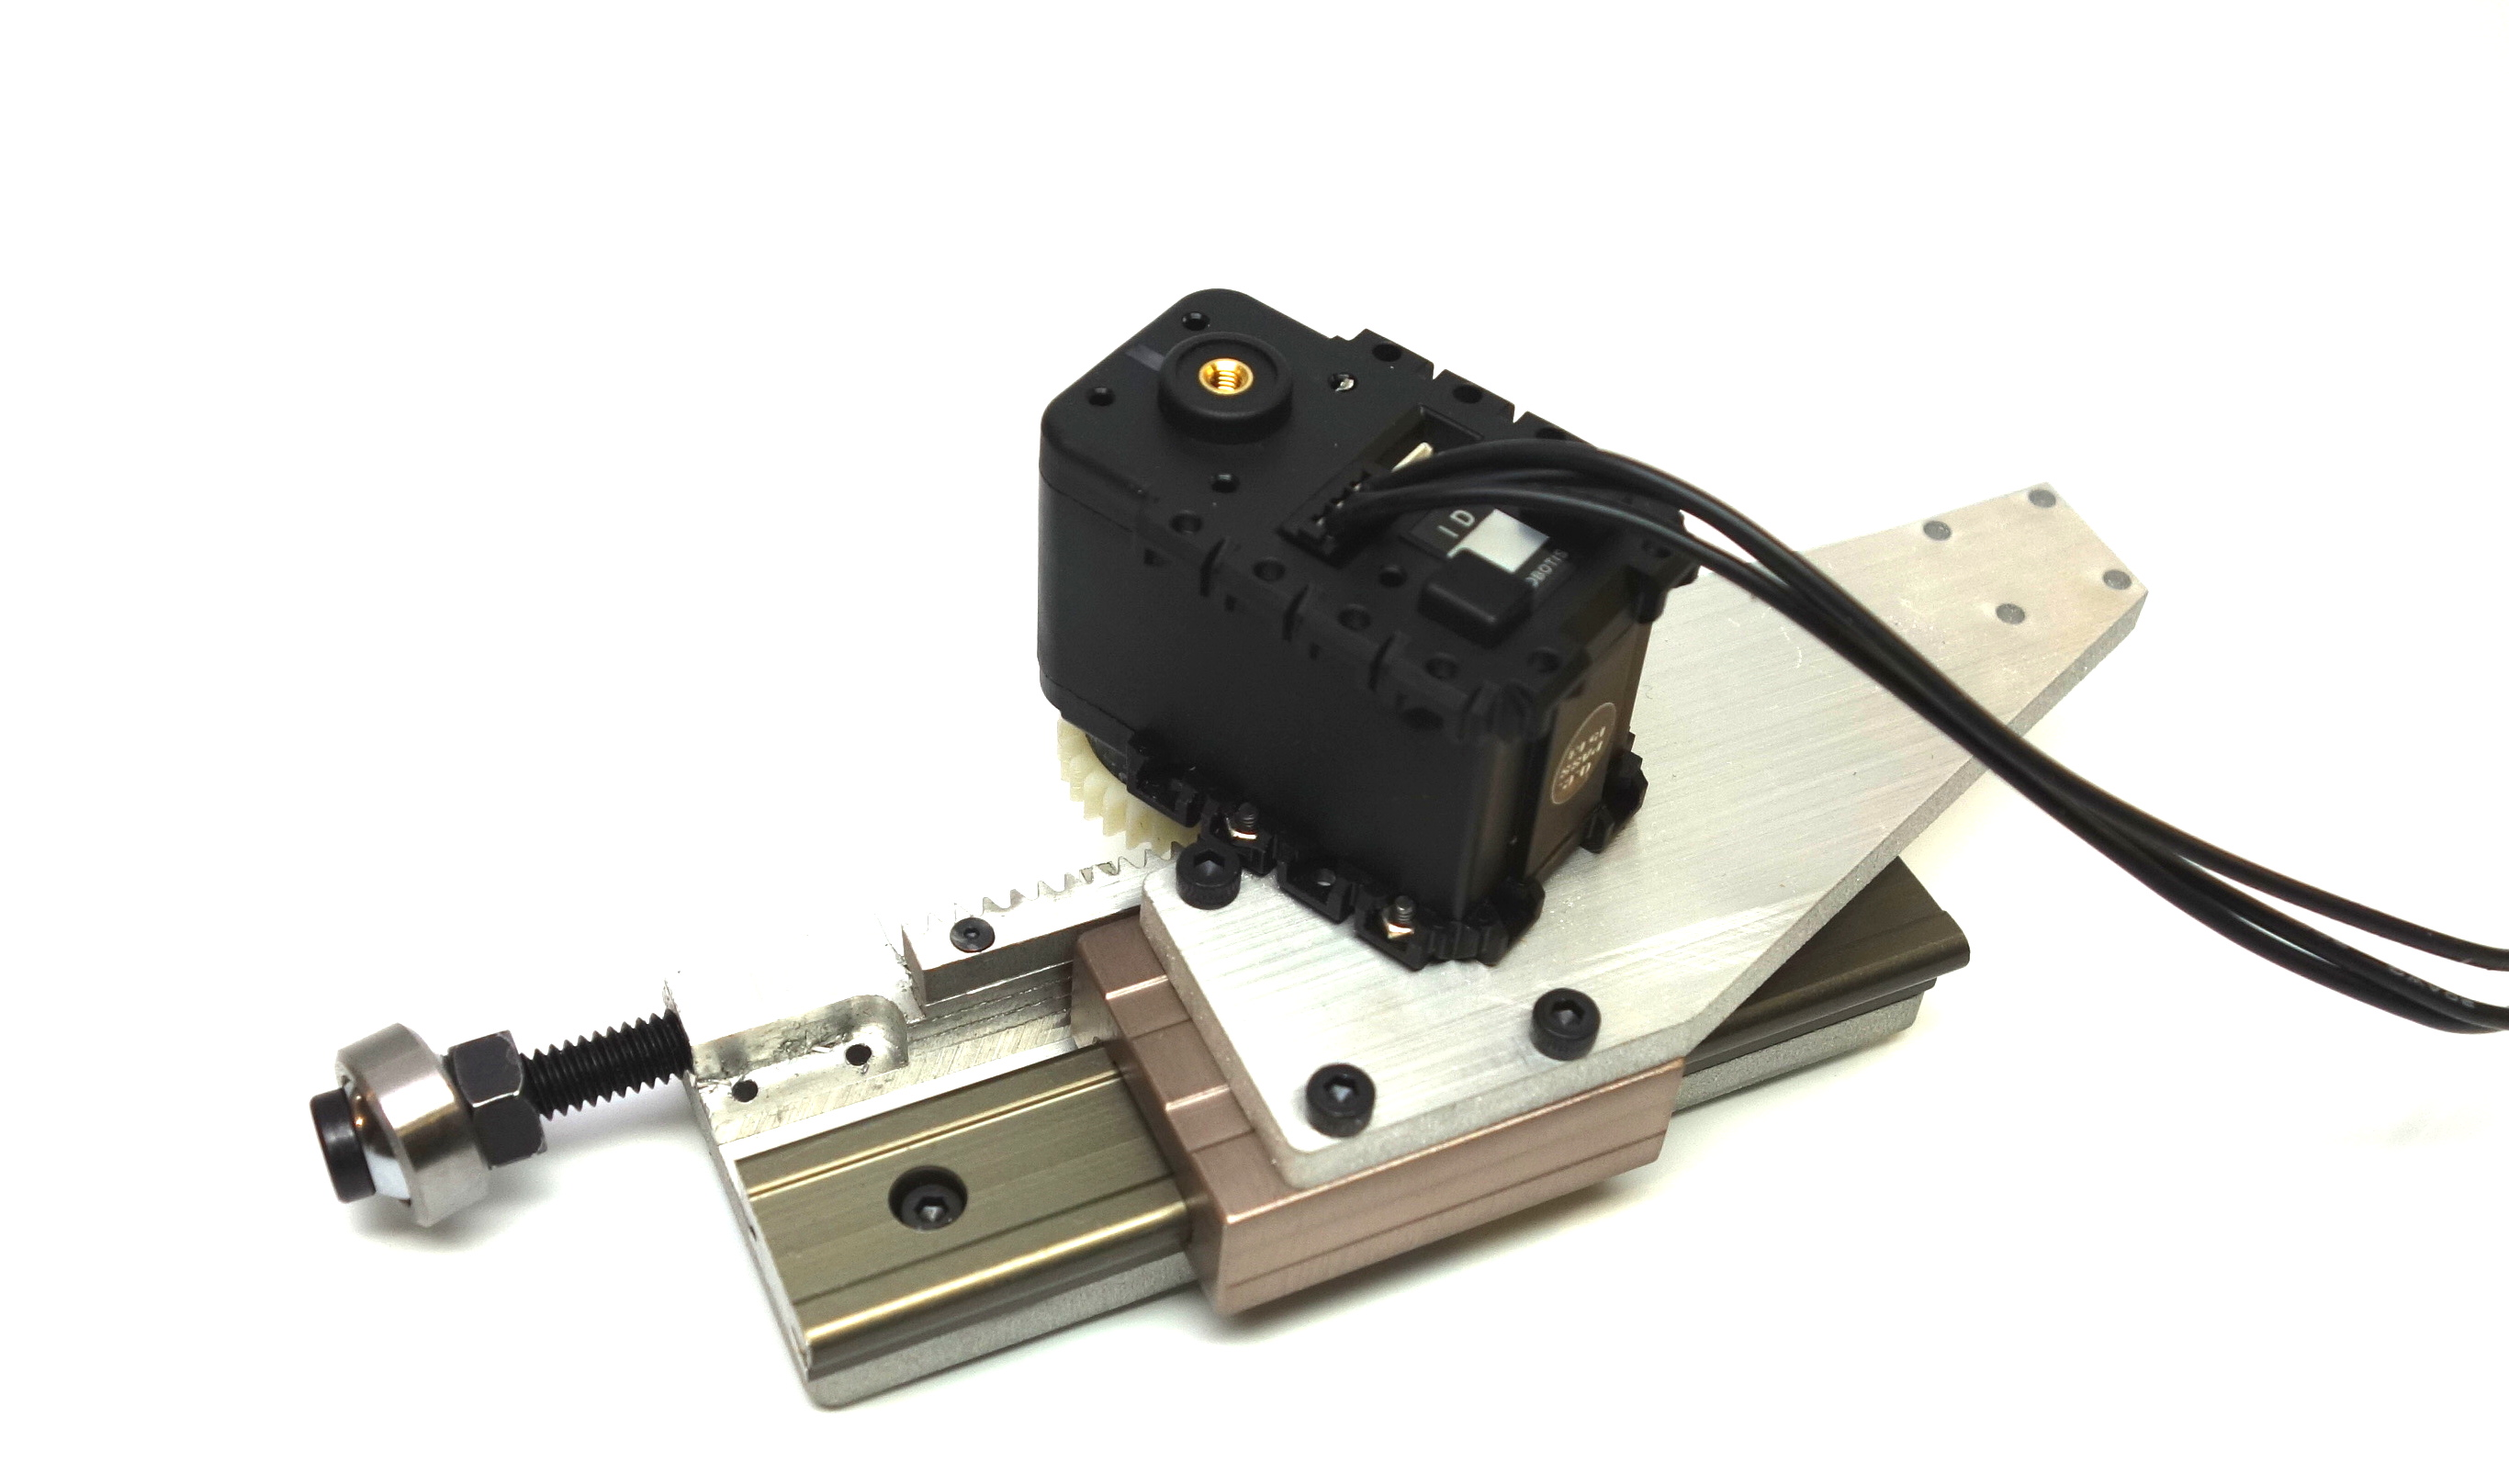
\includegraphics[width=4.6in]{figures/design/actuator.jpg}
      \caption{Detail of the linear actuator used to create squash-stretch animation in the robot's body}
      \label{fig_design_actuator}
   \end{figure}




   \begin{figure}[thpb]
      \centering
      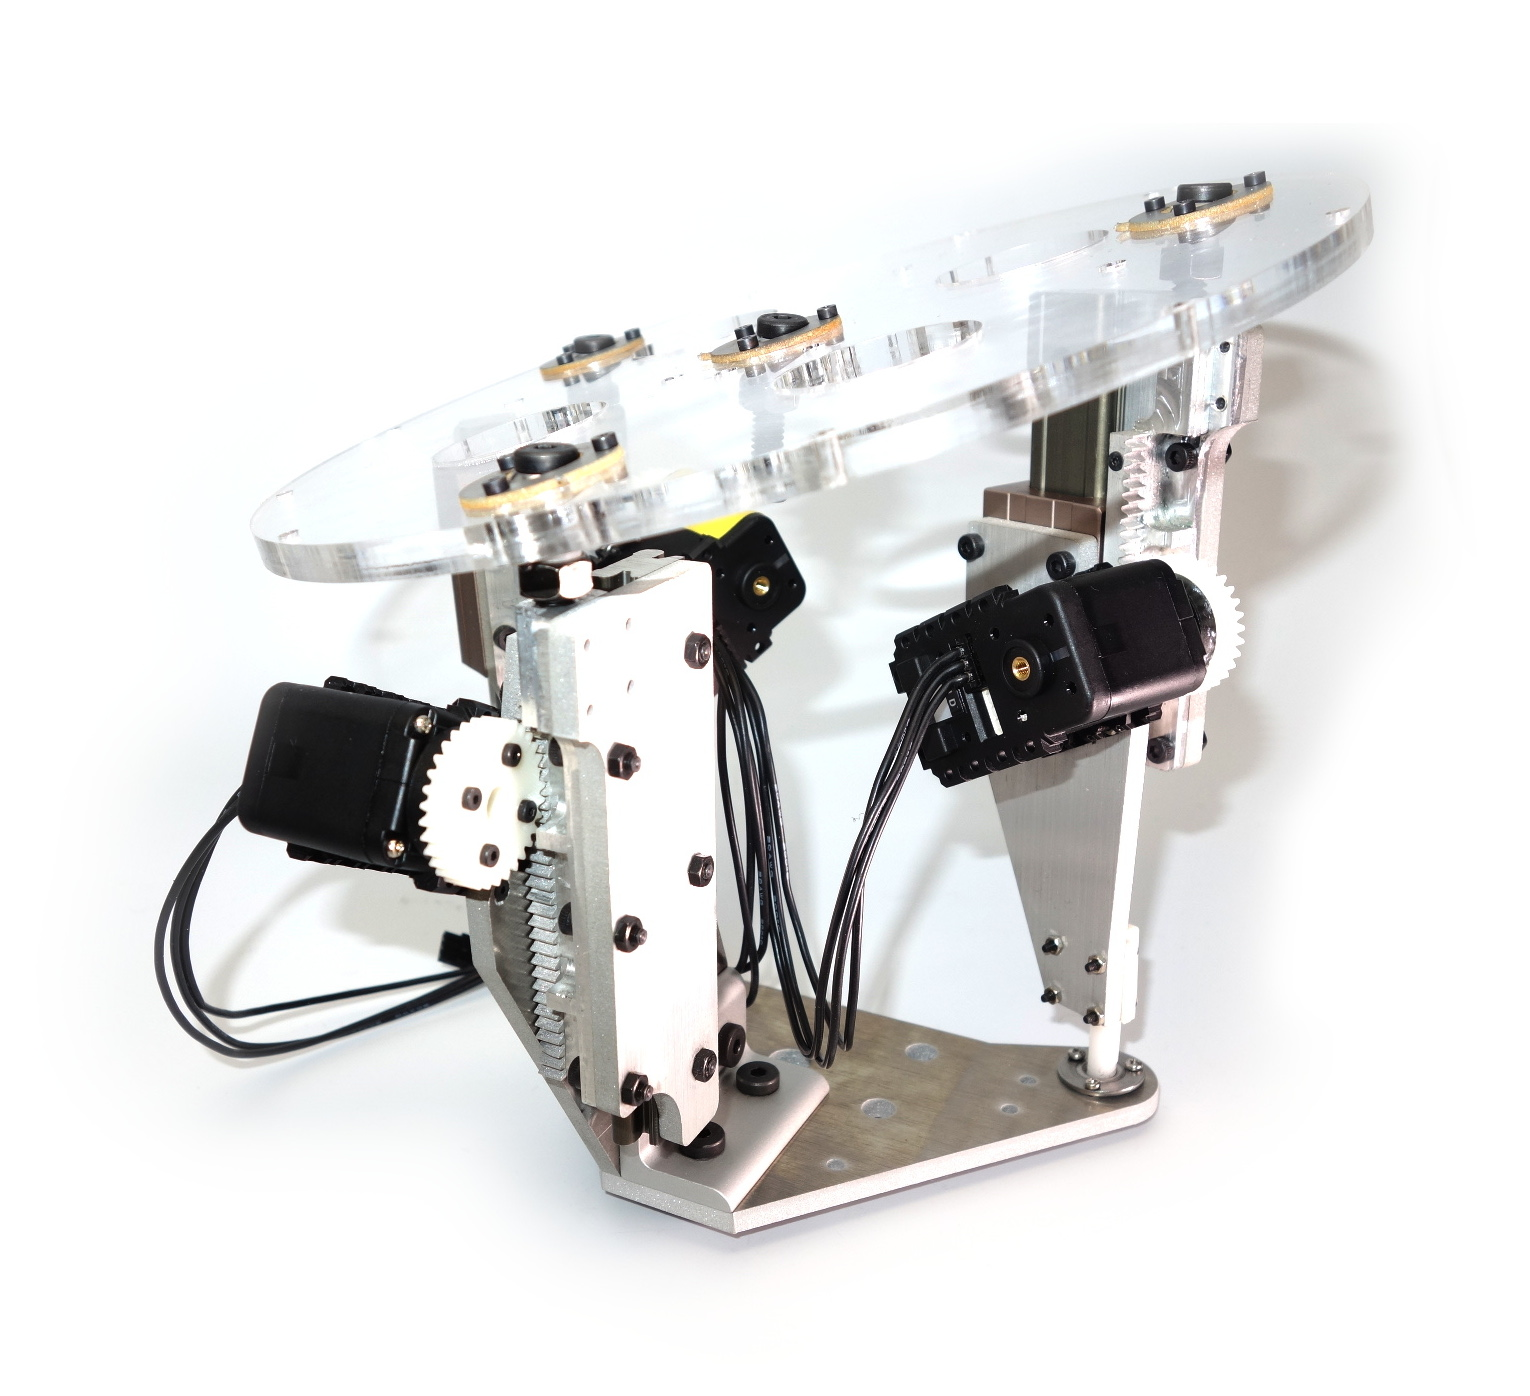
\includegraphics[width=4.6in]{figures/design/body_assem2.jpeg}
      \caption{Body assembly showing the top and bottom plates separated by the actuators}
      \label{fig_design_body_assem}
   \end{figure}





The linear actuators use a rack-and-pinion mechanism to translate the rotation of the motors into linear motion.\marginpar{

      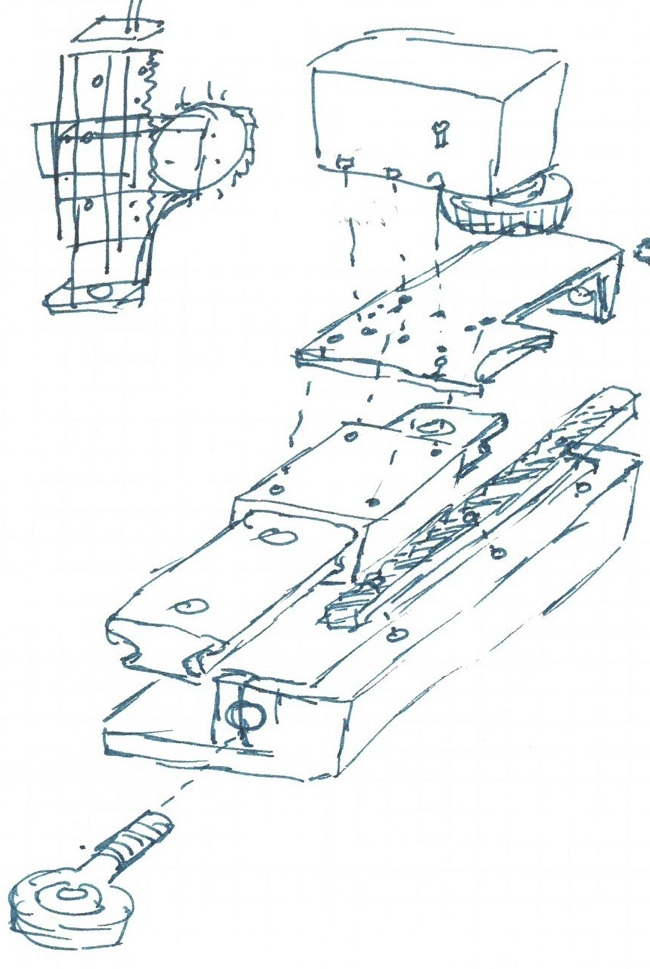
\includegraphics[width=\marginparwidth]{figures/design/linear_bearing_me_sketch.jpg}
      Sketch used as starting point for CAD drawing.
      %\caption{Juvenile owl used as an inspiration for the sound robot's form design.}
      \label{fig_design_linear_bearing}

   

} I made the frame and power transmission mechanism out of stock 6061 aluminum using a combination of waterjet and CNC. Off-the-shelf linear bearings constrain the motion to only one degree of freedom. Ball and swivel bearings connect each actuator to the plates above and below, which allows the plates to tilt relative to the actuator. Gravity preloads the pinion, so there is no backlash during normal operation. I used Dynamixel AX-12A servos for the motors, due to the absolute position control they provide over a serial bus. 



   \begin{figure}[thpb]
      \centering
      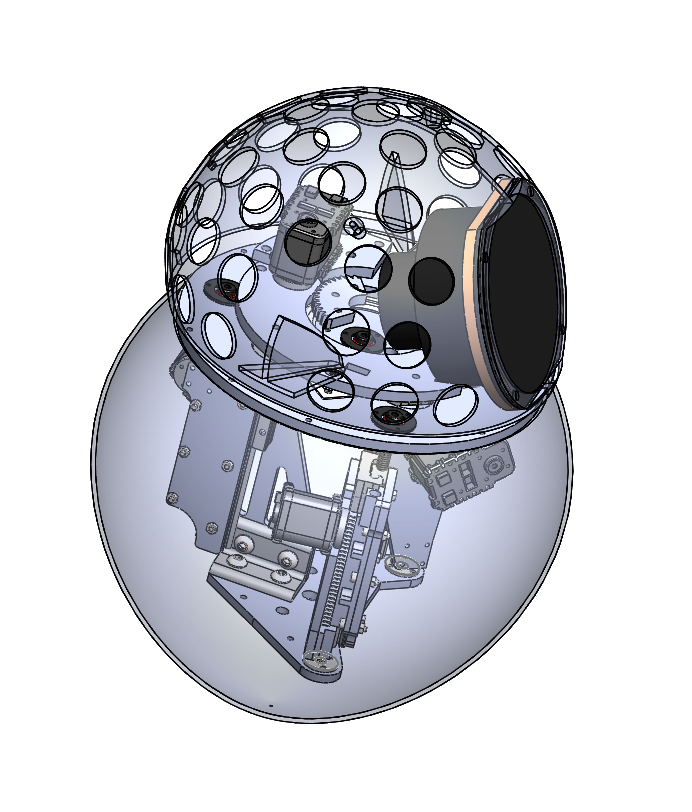
\includegraphics[width=4.6in]{figures/design/solidworks_body.png}
      \caption{CAD Drawings of my robot showing the actuators connecting the body plates. Head shows the speaker assembly and the rotation servo}
      \label{fig_design_solidworks}
   \end{figure}



The head, mounted on turntable bolted to the top plate of the body, can rotate through 120 degrees using another AX-12 servo. The forward tilt of the body of the robot puts the head on a canted axis, which creates a sweeping motion for the rotation of the head. Laser cut acrylic mounts in the head hold up a speaker, a full spectrum 4" Tang Tang Band W4­1320SJ driver, which forms the main visible feature of the face. 

\subsection{Skin}

The body of the robot is sheathed in bands of white craft foam that come to a point at the tail of the robot. The foam strips bellow out when the body plates contract creating the impression of organic mass. The head of the robot is encased in a 3D printed dome perforated with holes to reduce weight and cost. The overall form is suggestive of a juvenile owl. The gaps in the white foam and dome expose the internal mechanical structure of transparent acrylic and aluminum scaffolding. I intended to cover the foam and the dome with fur or feather boa to make the appearance more creature-like. However,  reaction to the accidental Bauhaus aesthetic of the robot was positive, so I decided to keep the robot in its semi-mechanical semi-organic form. 

\subsection{Electronics}

The electronics of the robot consists of a motor controller and an amplifier. The Dynamixel servos from the actuators and the head connect via daisy chained serial lines to an Arbotix controller located in the base of the robot. The controller, based on a AVR AtMega processor, talks to an off-board computer using a FTDI serial connection. The servos have on-board electronics for feedback position control so the main task of the controller is to provide power to the servos and adapt the servo serial communication to serial USB. 

The speaker is driven by a Sure TDA7492 Class D audio amplifier located alongside the motor controller. The amplifier routes the audio output of the computer to the robot speaker. A USB microphone provides audio input. The microphone array of a disassembled Microsoft Kinect provided audio localization but the feature was not used in the study. 

For the validation study, I made a fake memory card reader which consists of a 3D printed device that holds a memory stick shaped acrylic against a limit switch. The motor controller also provides an interface for digital sensing which is used to sense the presence of the memory stick.

The overall cost of materials for the robot came to \$815 USD with the servos being the most expensive item at \$180 USD for the 4 motors. 

\section{Software}

 In the last section, I described how the robot moves via the operation of four servos. Here, I will describe the action system that uses those servos to create believable motion, the cognition system which acts on the world by requesting actions of the action system, and the perception system through which cognition senses the world. These systems are connected together over Robot Operating System (ROS) \cite{ros}. I wrote these software components that run on the computer in Python. 


\subsection{Action System}


   \begin{figure}[thpb]
      \centering
      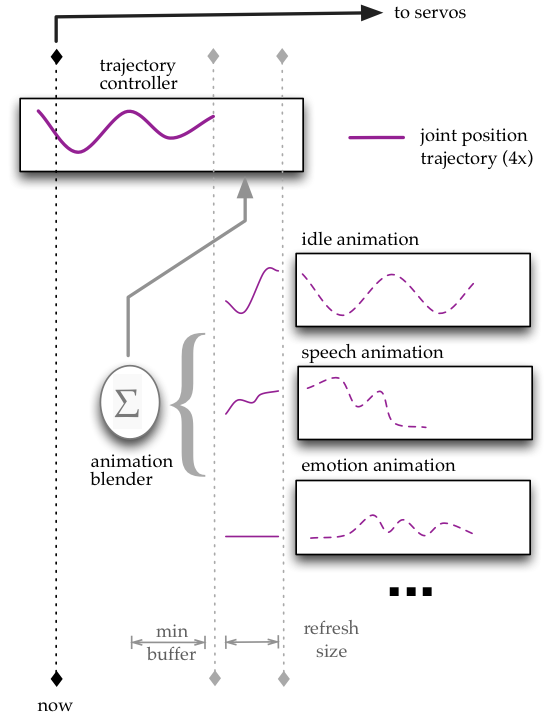
\includegraphics[width=4in]{figures/design/animation_system.png}
      \caption{Diagram showing the different components of the robot's action system. The trajectory controller sends position to the servos from a buffer of joint positions. When the buffer falls below a minimum threshold, the action system refreshes the buffer with blended chunks of trajectories from each submodule. The submodules maintain their own buffer of future trajectories. The buffer sizes are tuned to trade off reliable smoothness of animation with responsiveness.}
      \label{fig_animation_system}
   \end{figure}


The action system is the most complex part of the software, consisting of many threads of execution running in parallel (See Figure \ref{fig_animation_system}). At the lowest level of action is a feedback control loop running on each Dynamixel servo that, given a target position, will hold the motor at that position. Firmware on the Arbotix controller relays commands received over the serial link from the computer to the servos in the actuators and in the head.

On the computer, the Joint Trajectory Controller\footnote{I modified an existing controller by Vanadium Labs to allow the continuous buffering needed for smooth motion.} continuously sends target positions to the servos over the serial link. As an input, this controller takes in a trajectory, that is a series of positions for all of the robot's joints over a time window. On every clock tick, the controller interpolates positions and velocities and sends updates for the target position to the servos. To avoid discontinuity in the trajectory and keep the motion smooth, the controller maintains a buffer of joint positions. The action module, which is responsible for generating the joint trajectories, sends a new trajectory if the buffer falls below a minimum threshold. 

The action module forms the core of the action system. The module consists of separate submodules for each kind of action all running independently in parallel. For instance, an Idle Action submodule generates a breathing motion for the robot. Irrespective of other co-occuring actions, it creates a gentle expansion and contraction of the front of the robot. When the robot speaks, the Speaking Action submodule generates a motion trajectory to puff up the `chest' based on the energy of the utterance. There exist other submodules for producing emotionally expressive motions, for looking around, for playing back prerecorded animations, and so on. Each submodule maintains its own buffer of trajectories. When the controller's buffer gets low, the action module asks for small chunk of trajectories from each submodule, blends them together and then ships them over to the controller to extend its buffer. The blending allows the robot to continue breathing while speaking and turning its head. 

The action system works autonomously unless the cognition system requests a change in behavior. Each submodule of the action module exposes an interface over ROS so that cognition can trigger actions or changes in behavior of the submodules.

\subsection{Cognition System}

The cognition system reacts to the world as seen through the perception system and expresses itself through the action modules.  

The main task of cognition system for this robot is learning to speak from hearing people talk to it, and simply overhearing conversations. Per my thesis, the utterances the robot makes should be suggestive of the sounds it heard and engage the listener in reconstructing its experiences. The learning should occur quickly enough so that a casual human teacher would remain engaged through a training session. There is also the problem of people discovering the scope of the robot's experience: how would a new user of the robot know what it can say? While occasional random utterances of previously heard sounds wouldn't be entirely unlike the behavior of parrots, it would make the discovery of the robot's experience challenging. To help an user probe and explore the robot's experience, the robot should learn not just phrases but responses to phrases. 

There are two kinds of learning mechanism in the cognition system. With the first, the robot gets progressively better at mimicking a phrase it hears repeatedly; the second is how it learns responses to phrases. 

The first kind of learning is achieved through a simple pseudo-development mechanism\footnote{As an initial approach, I tried to approximate sounds heard by controlling the parameters of a simple vocal apparatus of sine wave generators. A Nelder Mead based gradient descent on the distance between the sound produced and target sound in a MFCC feature space, drives the utterances closer to target sound. While this mechanism, inspired by neurological understanding of song generation in zebra finches \cite{doya_computational_model_songbird}, is more biologically plausible, the optimization required many iterations in practice and was too slow to be useful for my application.} . A speech recognition engine in the cloud translates sounds from the environment into text where possible. The robot then repeats what it heard using a text-to-speech engine with some distortion to make its speech sound bird-like. A low-pass filter cuts off the high frequency sounds and the resulting sound is then pitch shifted up. The theshold and the degree of pitch shifting depends on the level of distortion ($threshold = 500 + (3500 * (1 - distortion))$; $shift percentage = 700 + (900 * distortion))$). The cognition system maintains a memory of all the phrases it heard and their frequency of repetition. As a phrase is heard more often, the distortion in the reproduction is progressively lowered making the utterance clearer. However, reproduction is never perfect and that combined with errors in speech recognition leaves some ambiguity about the utterance. The ambiguity was deliberate to engage the user in reconstructing the sound. 

The learning of responses to phrases is done using hebbian learning. The robot keeps track of phrases that frequently co-occur in conversations directed to it or that it overhears. For instance, the question ``What's up?'' might be followed by ``Not much'' or, perhaps more reflective of the exigencies of a center of learning and research, ``Aargh! I have a paper due.'' From this exchange the cognition system will maintain a link between ``What's up?'' and the example follow-on phrases. The robot will subsequently utter a follow-on phrase when it hears the antecedent. If there are many candidate phrases, cognition picks one with a probability based on the strength of association with the antecedent. 

The cognition also triggers various animations based on its state. For example, when it fails to transcribe speech, it triggers a mild head shaking animation through the action system. When cognition perceives an user is starting to talk to the robot, it causes the body to lean forward to express interest.  

For the purpose of the validation study, cognition also handled behavior associated with memory loss. When the memory of the robot is erased, it engaged in a distressed thrashing animation followed by a state where it responded to spoken phrases only by beeping. 

Lastly, there is a hidden command mode in the cognition system used for debugging and low level control of the robot. On hearing a key phrase, ``Joshua'', the robot transitions into this access mode. Then, using voice command an user can ask the robot to shutdown, to perform backups of memory, or to play a game of chess. 

\subsection{Perception System}

Being a sound robot, the primary perception of the robot is through the microphone. The robot looks for high energy in the audio stream and starts recording until pause at which point, it sends the recorded buffer to be converted to text using Google's speech recognition API. The cognition system responds to energy of the sound and the generated text. There is also mechanism for locating direction of sound using Microsoft Kinect's microphone array.

For the validation study, there were two more sources of input. An off-board hidden camera detected if there was  a face in the robot's view using a Haar cascade classification of the video stream. This mechanism was used to selectively engage the robot during a conversation with a study participant and to prevent the robot from interrupting the study with its utterances. In addition, the robot is wired to a limit sensor that detects the presence of a fake memory card. I will discuss the usage of these in the next chapter. 



In the next chapter, we will look at the results of human subject studies to determine people's perception of the robot, and particularly its ability to elicit empathy.














% 4-10 home
% 4-11 home
% 4-14 work

